\subsection{Folgeregelung}
        % Die LQR-Formulierung löst nur das Regulator Problem, wir können die Linearität des Systems ausnützen um einen gewünschten Zustand $x_{\infty}$ anzusteuern. 
        
        \textbf{Zur Erinnerung:} Ein lineares System beschreibt die Dynamik der Differenzen. Wir können den Ursprung des Systems demnach in einen neuen Punkt verschieben, mit den Definitionen $\Delta x = x -x_\infty$ und $\Delta u = u - u_\infty.$ Die Dynamik des Systems in den neuen Variablen lautet:
        \[\Delta\dot x = A \cdot \Delta x + B \cdot \Delta u,\]
        Wobei die Kostenfunktion nun auch angepasst werden muss:
        \[J(\Delta u) = \int^\infty_0(\Delta x^T(t) \cdot Q \cdot \Delta x(t) + \Delta u^T(t) \cdot R \cdot \Delta u(t)) dt \]
        das neue Regulator Problem lautet somit: 
        \[\lim\limits_{0 \to \infty} \Delta x(t) = 0 \]
        Somit linearisiert man das System um einen neuen Punkt $\{x_\infty,u_\infty\}$. Dies eintspricht bei einem linearen System ein Ursprungsverschiebung. Die Lösung des Regulatorsproblems der Dynamik der Differenz lautet nun
        \[\Delta u = u - u _\infty = -K \cdot \Delta x = -K \cdot ( x-x_\infty)\]
        Der Eingang auf das originale System $\dot x = A\cdot x + B \cdot u$ lautet somit:
        \[u = u_\infty - K \cdot (x-x_\infty),\]
        wobei $u_\infty$ ein statisches feedforward Signal ist, welches das System am gewünschten Punkt $x_\infty$ hält. 
        
        Im Gleichgewicht sind alle Ableitungen null: \[ 0 = A\cdot x_{\infty} + B \cdot u_\infty\]
        
        \begin{figure}[H]
            \centering
            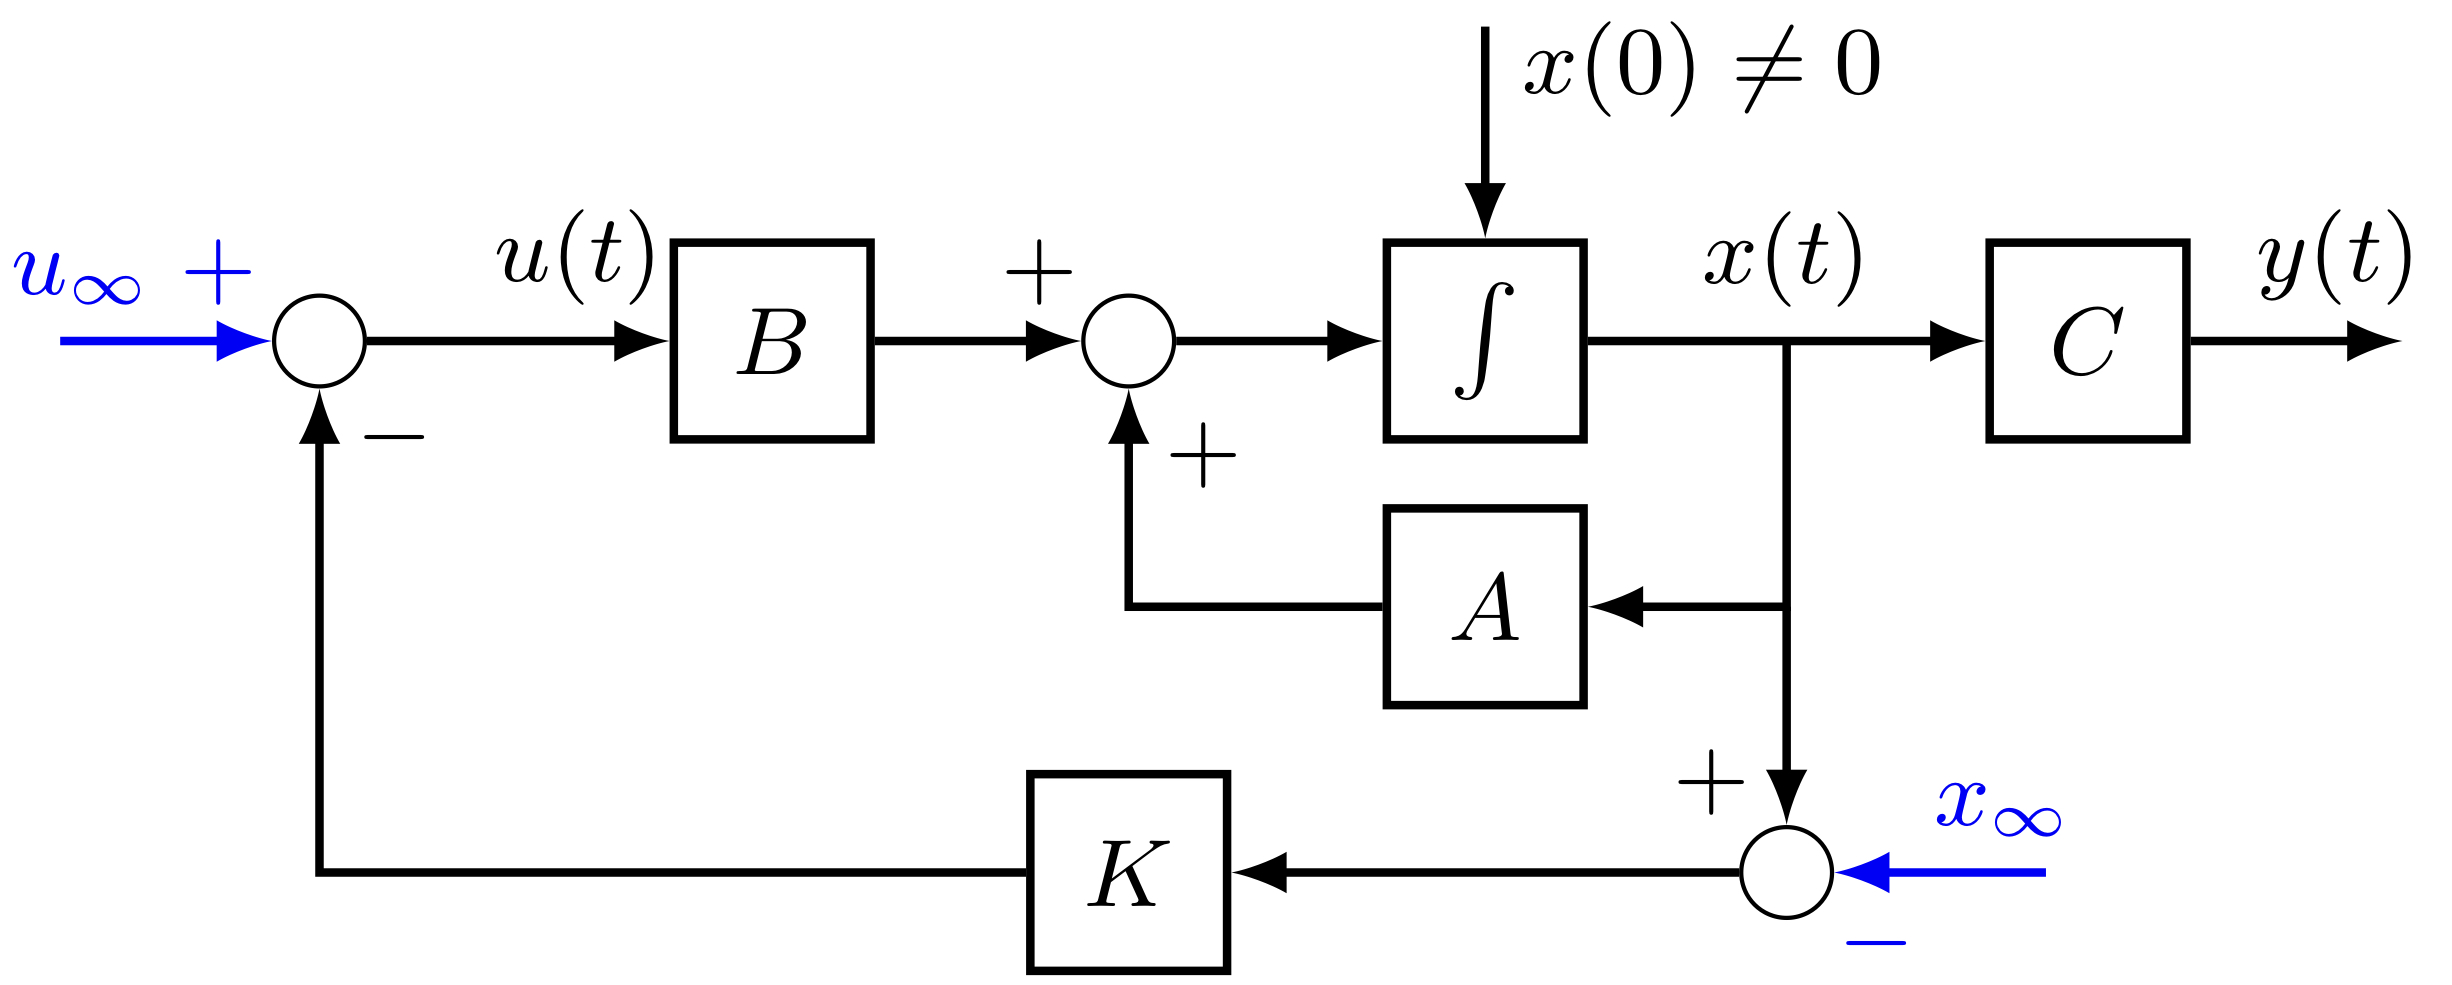
\includegraphics[width = 0.8\linewidth]{images/08/LQR_Folgeregelung.jpeg}
        \end{figure}
        
        \textbf{Bemerkungen}:
        \begin{itemize}
            \item Die Stellgrösse $u_\infty$ ist statisch für eine statische Referenz $x_\infty$. 
            \item Die Folgeregelung mit feedforward kann keine Störungen unterdrücken.
            \end{itemize}